\section{Evaluation}
\label{sec:Evaluation}
\subsection{Application of Principal Component Analysis}
\label{sub:ApplicationofPrincipalComponentAnalysis}
As mentioned in Section~\ref{sub:Experiment} - \nameref{sub:Experiment}, we have four types of scenarios --
all of which we had tried to analyse to find principal components.
For each different types of scenario, we will in the following sections discuss the process of picking the principal components for analysis, what the result of the analysis is, and
how we use the generative ability of PCA to examine what each component represent variance of.

\subsubsection{Picking Principal Components}
\label{ssub:PickingPrincipalComponents}
Usually the first task after extracting principal components is to choose which of them to keep, depending on the needed variation. 
To visualize how much each principal component influenced the variation, we have plotted them using a bar chart that shows how much
of the total percentage each principal component composes (see Figure~\ref{fig:eigvplot}).
Furthermore we have plotted the cumulative sum to see how many principal components we need to have a certain percentage of variation.\\

  \begin{minipage}{\linewidth}
  \centering
  \makebox[\linewidth] {
  \begin{tabular}{cc}
      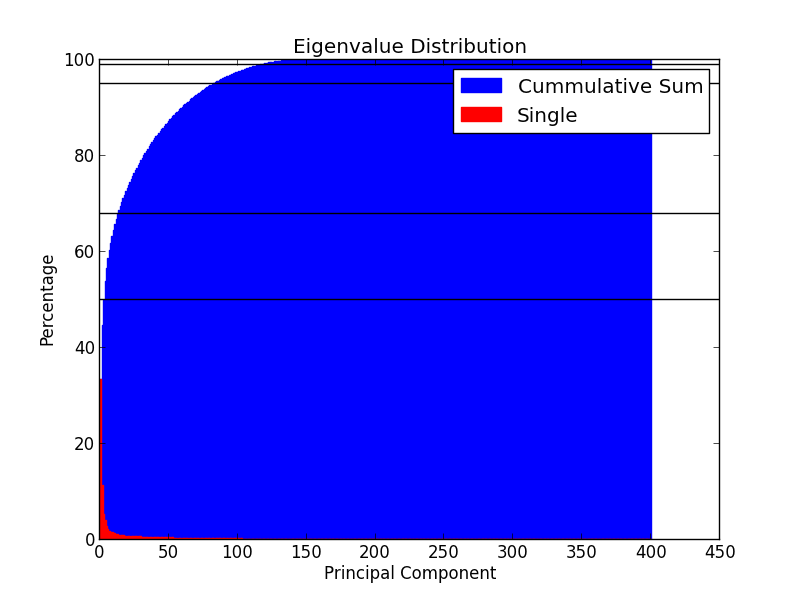
\includegraphics[width=0.5\textwidth]{NLHM-Eigenvalueplot.png}
    & 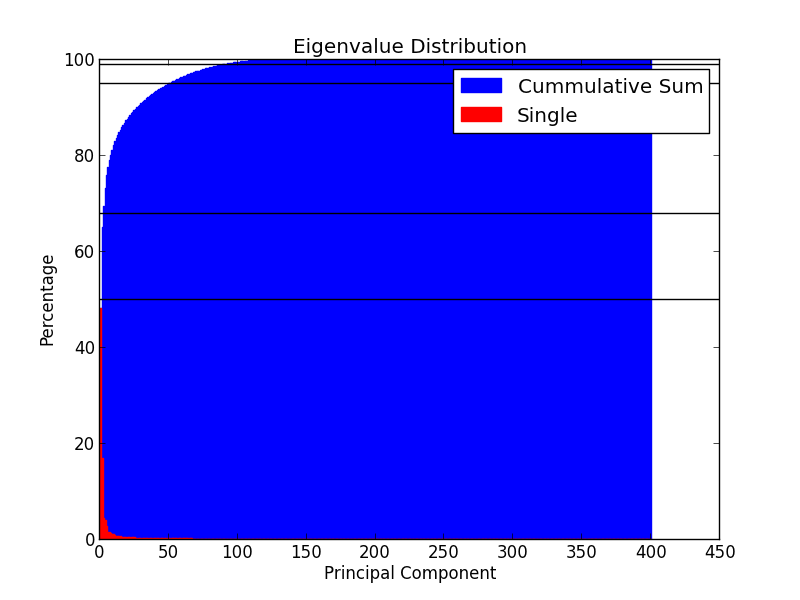
\includegraphics[width=0.5\textwidth]{NLHS-Eigenvalueplot.png} \\
      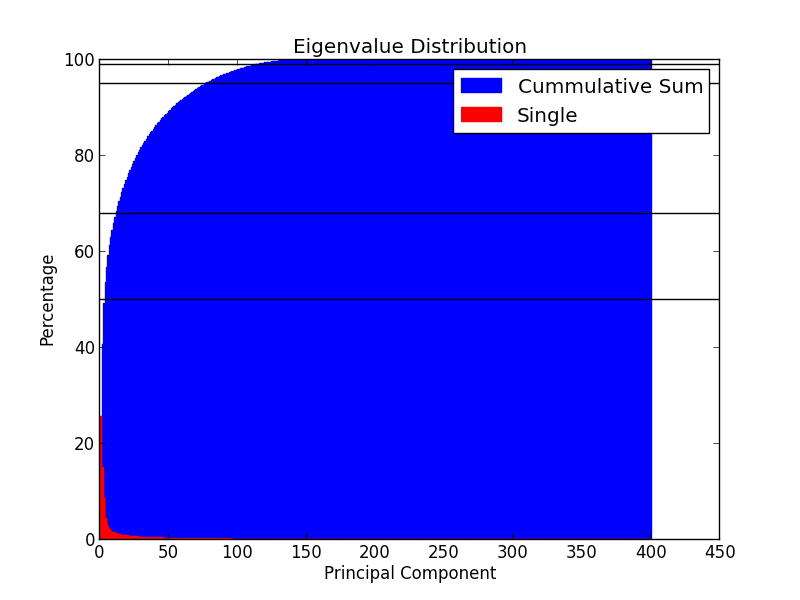
\includegraphics[width=0.5\textwidth]{WLHM-Eigenvalueplot.png}
    & 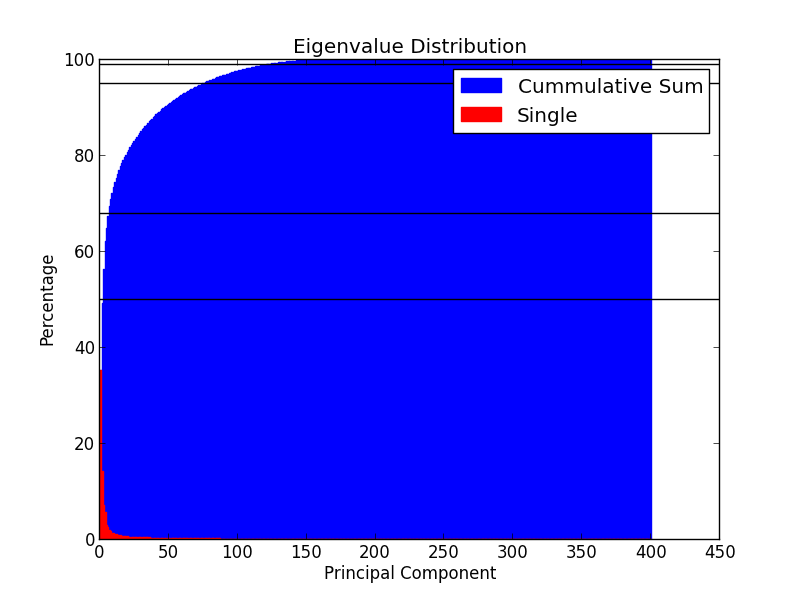
\includegraphics[width=0.5\textwidth]{WLHS-Eigenvalueplot.png}
  \end{tabular}
  }
  \captionof{figure}{Principal Components - Distribution of Variance using Eigenvalues\\
  (Left --- Right: Head Move --- Head Still, Up --- Down: No Light --- With Light)}\label{fig:eigvplot}
  \end{minipage}\\\\

As may be seen in the plots (Figure~\ref{fig:eigvplot}), in all of our test cases the first few (5-7) principal components compose almost
50\% of variation.
What is yet more interesting is that to get almost 95\% of the variation, we need almost 70 principal components in every case.
This might seem as an unusually high number, because a lot of the variations that compose the variation between 50-95\% are small in size, yet
they accumulate in size.
A possible explanation could be that our images have a lot of small variation on light, eye movement and appearance (e.g. eye colour, iris shape, etc.),
which might not useful for our purpose. This is a trade-off inherent of PCA, because it is a statistical and unsupervised method, and some of the data output
might be considered noise.

While we had examined the individual plots of all principal components to ensure that we did not exclude anything of interest, we chose to only use the most important 5 in Section~\ref{ssub:ResultData}.
This is due to the fact that while they do not represent almost all variation, they represented a comprehensible number of features while
still having a large majority. Furthermore as we will see in the next section, the features which we can use for classification, i.e. that are separable in the groups we have, are
only represented in the most important principal components.

\subsubsection{Generative Image Representation}
\label{ssub:GenerativeImageRepresentation}

To better understand what each of the most important principal components, represent we have used the generative abilities of PCA 
to look at the variation of the eye images.\\

  \begin{minipage}{\linewidth}
  \centering
  \makebox[\linewidth] {
  \begin{tabular}{ccccccc}
      \includegraphics[width=0.1\textwidth]{GeneratedImages/NLHM/PCA0-SIGMA-3.jpg}
    & \includegraphics[width=0.1\textwidth]{GeneratedImages/NLHM/PCA0-SIGMA-2.jpg}
    & \includegraphics[width=0.1\textwidth]{GeneratedImages/NLHM/PCA0-SIGMA-1.jpg}
    & \includegraphics[width=0.1\textwidth]{GeneratedImages/NLHM/PCA0-SIGMA0.jpg}
    & \includegraphics[width=0.1\textwidth]{GeneratedImages/NLHM/PCA0-SIGMA1.jpg}
    & \includegraphics[width=0.1\textwidth]{GeneratedImages/NLHM/PCA0-SIGMA2.jpg}
    & \includegraphics[width=0.1\textwidth]{GeneratedImages/NLHM/PCA0-SIGMA3.jpg} \\
      \includegraphics[width=0.1\textwidth]{GeneratedImages/NLHM/PCA1-SIGMA-3.jpg}
    & \includegraphics[width=0.1\textwidth]{GeneratedImages/NLHM/PCA1-SIGMA-2.jpg}
    & \includegraphics[width=0.1\textwidth]{GeneratedImages/NLHM/PCA1-SIGMA-1.jpg}
    & \includegraphics[width=0.1\textwidth]{GeneratedImages/NLHM/PCA1-SIGMA0.jpg}
    & 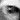
\includegraphics[width=0.1\textwidth]{GeneratedImages/NLHM/PCA1-SIGMA1.jpg}
    & 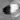
\includegraphics[width=0.1\textwidth]{GeneratedImages/NLHM/PCA1-SIGMA2.jpg}
    & 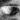
\includegraphics[width=0.1\textwidth]{GeneratedImages/NLHM/PCA1-SIGMA3.jpg} \\
      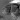
\includegraphics[width=0.1\textwidth]{GeneratedImages/NLHM/PCA2-SIGMA-3.jpg}
    & 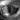
\includegraphics[width=0.1\textwidth]{GeneratedImages/NLHM/PCA2-SIGMA-2.jpg}
    & 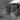
\includegraphics[width=0.1\textwidth]{GeneratedImages/NLHM/PCA2-SIGMA-1.jpg}
    & 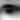
\includegraphics[width=0.1\textwidth]{GeneratedImages/NLHM/PCA2-SIGMA0.jpg}
    & 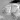
\includegraphics[width=0.1\textwidth]{GeneratedImages/NLHM/PCA2-SIGMA1.jpg}
    & 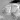
\includegraphics[width=0.1\textwidth]{GeneratedImages/NLHM/PCA2-SIGMA2.jpg}
    & 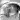
\includegraphics[width=0.1\textwidth]{GeneratedImages/NLHM/PCA2-SIGMA3.jpg} \\
      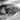
\includegraphics[width=0.1\textwidth]{GeneratedImages/NLHM/PCA3-SIGMA-3.jpg}
    & 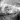
\includegraphics[width=0.1\textwidth]{GeneratedImages/NLHM/PCA3-SIGMA-2.jpg}
    & 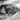
\includegraphics[width=0.1\textwidth]{GeneratedImages/NLHM/PCA3-SIGMA-1.jpg}
    & 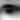
\includegraphics[width=0.1\textwidth]{GeneratedImages/NLHM/PCA3-SIGMA0.jpg}
    & 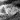
\includegraphics[width=0.1\textwidth]{GeneratedImages/NLHM/PCA3-SIGMA1.jpg}
    & 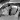
\includegraphics[width=0.1\textwidth]{GeneratedImages/NLHM/PCA3-SIGMA2.jpg}
    & 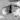
\includegraphics[width=0.1\textwidth]{GeneratedImages/NLHM/PCA3-SIGMA3.jpg} \\
      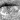
\includegraphics[width=0.1\textwidth]{GeneratedImages/NLHM/PCA4-SIGMA-3.jpg}
    & 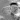
\includegraphics[width=0.1\textwidth]{GeneratedImages/NLHM/PCA4-SIGMA-2.jpg}
    & 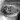
\includegraphics[width=0.1\textwidth]{GeneratedImages/NLHM/PCA4-SIGMA-1.jpg}
    & 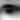
\includegraphics[width=0.1\textwidth]{GeneratedImages/NLHM/PCA4-SIGMA0.jpg}
    & 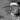
\includegraphics[width=0.1\textwidth]{GeneratedImages/NLHM/PCA4-SIGMA1.jpg}
    & 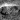
\includegraphics[width=0.1\textwidth]{GeneratedImages/NLHM/PCA4-SIGMA2.jpg}
    & 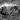
\includegraphics[width=0.1\textwidth]{GeneratedImages/NLHM/PCA4-SIGMA3.jpg}
  \end{tabular}
  }
  \captionof{figure}{No Light Head Move -- Generated PCA Images (Up --- Down: PC 1 --- PC 5, Left --- Right: -3$\sigma$ --- 3$\sigma$)}\label{fig:nlhmpcaimages}
  \end{minipage}\\\\

  In our NLHM dataset it seems that the most important principal component is the second one, as it represents the variation of the looking direction (See Figure~\ref{fig:nlhmpcaimages}).
  Interestingly, the principal component with most variation seem to relate to lighting conditions, even though our training data stems from the same room.
  The final principal components does not seem to be of interest as they seem to represent eye color, and different types of eyelid movements respectively.\\

  \begin{minipage}{\linewidth}
  \centering
  \makebox[\linewidth] {
  \begin{tabular}{ccccccc}
      \includegraphics[width=0.1\textwidth]{GeneratedImages/NLHS/PCA0-SIGMA-3.jpg}
    & \includegraphics[width=0.1\textwidth]{GeneratedImages/NLHS/PCA0-SIGMA-2.jpg}
    & \includegraphics[width=0.1\textwidth]{GeneratedImages/NLHS/PCA0-SIGMA-1.jpg}
    & \includegraphics[width=0.1\textwidth]{GeneratedImages/NLHS/PCA0-SIGMA0.jpg}
    & \includegraphics[width=0.1\textwidth]{GeneratedImages/NLHS/PCA0-SIGMA1.jpg}
    & \includegraphics[width=0.1\textwidth]{GeneratedImages/NLHS/PCA0-SIGMA2.jpg}
    & \includegraphics[width=0.1\textwidth]{GeneratedImages/NLHS/PCA0-SIGMA3.jpg} \\
      \includegraphics[width=0.1\textwidth]{GeneratedImages/NLHS/PCA1-SIGMA-3.jpg}
    & \includegraphics[width=0.1\textwidth]{GeneratedImages/NLHS/PCA1-SIGMA-2.jpg}
    & \includegraphics[width=0.1\textwidth]{GeneratedImages/NLHS/PCA1-SIGMA-1.jpg}
    & \includegraphics[width=0.1\textwidth]{GeneratedImages/NLHS/PCA1-SIGMA0.jpg}
    & \includegraphics[width=0.1\textwidth]{GeneratedImages/NLHS/PCA1-SIGMA1.jpg}
    & \includegraphics[width=0.1\textwidth]{GeneratedImages/NLHS/PCA1-SIGMA2.jpg}
    & \includegraphics[width=0.1\textwidth]{GeneratedImages/NLHS/PCA1-SIGMA3.jpg} \\
      \includegraphics[width=0.1\textwidth]{GeneratedImages/NLHS/PCA2-SIGMA-3.jpg}
    & \includegraphics[width=0.1\textwidth]{GeneratedImages/NLHS/PCA2-SIGMA-2.jpg}
    & \includegraphics[width=0.1\textwidth]{GeneratedImages/NLHS/PCA2-SIGMA-1.jpg}
    & \includegraphics[width=0.1\textwidth]{GeneratedImages/NLHS/PCA2-SIGMA0.jpg}
    & \includegraphics[width=0.1\textwidth]{GeneratedImages/NLHS/PCA2-SIGMA1.jpg}
    & \includegraphics[width=0.1\textwidth]{GeneratedImages/NLHS/PCA2-SIGMA2.jpg}
    & \includegraphics[width=0.1\textwidth]{GeneratedImages/NLHS/PCA2-SIGMA3.jpg} \\
      \includegraphics[width=0.1\textwidth]{GeneratedImages/NLHS/PCA3-SIGMA-3.jpg}
    & \includegraphics[width=0.1\textwidth]{GeneratedImages/NLHS/PCA3-SIGMA-2.jpg}
    & \includegraphics[width=0.1\textwidth]{GeneratedImages/NLHS/PCA3-SIGMA-1.jpg}
    & \includegraphics[width=0.1\textwidth]{GeneratedImages/NLHS/PCA3-SIGMA0.jpg}
    & \includegraphics[width=0.1\textwidth]{GeneratedImages/NLHS/PCA3-SIGMA1.jpg}
    & \includegraphics[width=0.1\textwidth]{GeneratedImages/NLHS/PCA3-SIGMA2.jpg}
    & \includegraphics[width=0.1\textwidth]{GeneratedImages/NLHS/PCA3-SIGMA3.jpg} \\
      \includegraphics[width=0.1\textwidth]{GeneratedImages/NLHS/PCA4-SIGMA-3.jpg}
    & \includegraphics[width=0.1\textwidth]{GeneratedImages/NLHS/PCA4-SIGMA-2.jpg}
    & \includegraphics[width=0.1\textwidth]{GeneratedImages/NLHS/PCA4-SIGMA-1.jpg}
    & \includegraphics[width=0.1\textwidth]{GeneratedImages/NLHS/PCA4-SIGMA0.jpg}
    & \includegraphics[width=0.1\textwidth]{GeneratedImages/NLHS/PCA4-SIGMA1.jpg}
    & \includegraphics[width=0.1\textwidth]{GeneratedImages/NLHS/PCA4-SIGMA2.jpg}
    & \includegraphics[width=0.1\textwidth]{GeneratedImages/NLHS/PCA4-SIGMA3.jpg} \\

  \end{tabular}
  }
  \captionof{figure}{No Light Head Still -- Generated PCA Images (Up --- Down: PC 1 --- PC 5, Left --- Right: -3$\sigma$ --- 3$\sigma$)}\label{fig:nlhspcaimages}
  \end{minipage}\\\\

  Similarly to our NLHM dataset, our NLHS datasets first and second components seem to represent lighting and eye direction variation respectively (See Figure~\ref{fig:nlhspcaimages}).
  It seems hard to see what the variation of the last three component, but a qualified guess would be that they represent differences in iris colour and eye open-close movements. None of the last three principal components,
  seem to provide us with better support for doing gaze estimation.\\

  \begin{minipage}{\linewidth}
  \centering
  \makebox[\linewidth] {
  \begin{tabular}{ccccccc}
      \includegraphics[width=0.1\textwidth]{GeneratedImages/WLHM/PCA0-SIGMA-3.jpg}
    & \includegraphics[width=0.1\textwidth]{GeneratedImages/WLHM/PCA0-SIGMA-2.jpg}
    & \includegraphics[width=0.1\textwidth]{GeneratedImages/WLHM/PCA0-SIGMA-1.jpg}
    & \includegraphics[width=0.1\textwidth]{GeneratedImages/WLHM/PCA0-SIGMA0.jpg}
    & \includegraphics[width=0.1\textwidth]{GeneratedImages/WLHM/PCA0-SIGMA1.jpg}
    & \includegraphics[width=0.1\textwidth]{GeneratedImages/WLHM/PCA0-SIGMA2.jpg}
    & \includegraphics[width=0.1\textwidth]{GeneratedImages/WLHM/PCA0-SIGMA3.jpg} \\
      \includegraphics[width=0.1\textwidth]{GeneratedImages/WLHM/PCA1-SIGMA-3.jpg}
    & \includegraphics[width=0.1\textwidth]{GeneratedImages/WLHM/PCA1-SIGMA-2.jpg}
    & \includegraphics[width=0.1\textwidth]{GeneratedImages/WLHM/PCA1-SIGMA-1.jpg}
    & \includegraphics[width=0.1\textwidth]{GeneratedImages/WLHM/PCA1-SIGMA0.jpg}
    & \includegraphics[width=0.1\textwidth]{GeneratedImages/WLHM/PCA1-SIGMA1.jpg}
    & \includegraphics[width=0.1\textwidth]{GeneratedImages/WLHM/PCA1-SIGMA2.jpg}
    & \includegraphics[width=0.1\textwidth]{GeneratedImages/WLHM/PCA1-SIGMA3.jpg} \\
      \includegraphics[width=0.1\textwidth]{GeneratedImages/WLHM/PCA2-SIGMA-3.jpg}
    & \includegraphics[width=0.1\textwidth]{GeneratedImages/WLHM/PCA2-SIGMA-2.jpg}
    & \includegraphics[width=0.1\textwidth]{GeneratedImages/WLHM/PCA2-SIGMA-1.jpg}
    & \includegraphics[width=0.1\textwidth]{GeneratedImages/WLHM/PCA2-SIGMA0.jpg}
    & \includegraphics[width=0.1\textwidth]{GeneratedImages/WLHM/PCA2-SIGMA1.jpg}
    & \includegraphics[width=0.1\textwidth]{GeneratedImages/WLHM/PCA2-SIGMA2.jpg}
    & \includegraphics[width=0.1\textwidth]{GeneratedImages/WLHM/PCA2-SIGMA3.jpg} \\
      \includegraphics[width=0.1\textwidth]{GeneratedImages/WLHM/PCA3-SIGMA-3.jpg}
    & \includegraphics[width=0.1\textwidth]{GeneratedImages/WLHM/PCA3-SIGMA-2.jpg}
    & \includegraphics[width=0.1\textwidth]{GeneratedImages/WLHM/PCA3-SIGMA-1.jpg}
    & \includegraphics[width=0.1\textwidth]{GeneratedImages/WLHM/PCA3-SIGMA0.jpg}
    & \includegraphics[width=0.1\textwidth]{GeneratedImages/WLHM/PCA3-SIGMA1.jpg}
    & \includegraphics[width=0.1\textwidth]{GeneratedImages/WLHM/PCA3-SIGMA2.jpg}
    & \includegraphics[width=0.1\textwidth]{GeneratedImages/WLHM/PCA3-SIGMA3.jpg} \\
      \includegraphics[width=0.1\textwidth]{GeneratedImages/WLHM/PCA4-SIGMA-3.jpg}
    & \includegraphics[width=0.1\textwidth]{GeneratedImages/WLHM/PCA4-SIGMA-2.jpg}
    & \includegraphics[width=0.1\textwidth]{GeneratedImages/WLHM/PCA4-SIGMA-1.jpg}
    & \includegraphics[width=0.1\textwidth]{GeneratedImages/WLHM/PCA4-SIGMA0.jpg}
    & \includegraphics[width=0.1\textwidth]{GeneratedImages/WLHM/PCA4-SIGMA1.jpg}
    & \includegraphics[width=0.1\textwidth]{GeneratedImages/WLHM/PCA4-SIGMA2.jpg}
    & \includegraphics[width=0.1\textwidth]{GeneratedImages/WLHM/PCA4-SIGMA3.jpg} \\

  \end{tabular}
  }
  \captionof{figure}{With Light Head Move -- Generated PCA Images (Up --- Down: PA 1 --- PA 5, Left --- Right: -3$\sigma$ --- 3$\sigma$)}\label{fig:wlhmpcaimages}
  \end{minipage}\\\\

  The WLHM dataset seems to provide an interesting array of variation regarding the first couple of principal components (See Figure~\ref{fig:wlhmpcaimages}).
  It seems as though they represent the reflection of our infra-red lights, but as the head is moving it seems to be registered as blobs of light, instead
  of being separable individually. This obviously makes it harder to use this feature of our eye image directly, but may be utilized for normalization in different scenarios.
  The third principal component seems the most interesting one as it is the one representing eye direction variation, and as such this dataset specifically differs
  from the other (where the second principal component was the one used).\\ The last couple of principal components seem again to represent differences in eyelid movements.\\

  \begin{minipage}{\linewidth}
  \centering
  \makebox[\linewidth] {
  \begin{tabular}{ccccccc}
      \includegraphics[width=0.1\textwidth]{GeneratedImages/WLHS/PCA0-SIGMA-3.jpg}
    & \includegraphics[width=0.1\textwidth]{GeneratedImages/WLHS/PCA0-SIGMA-2.jpg}
    & \includegraphics[width=0.1\textwidth]{GeneratedImages/WLHS/PCA0-SIGMA-1.jpg}
    & \includegraphics[width=0.1\textwidth]{GeneratedImages/WLHS/PCA0-SIGMA0.jpg}
    & \includegraphics[width=0.1\textwidth]{GeneratedImages/WLHS/PCA0-SIGMA1.jpg}
    & \includegraphics[width=0.1\textwidth]{GeneratedImages/WLHS/PCA0-SIGMA2.jpg}
    & \includegraphics[width=0.1\textwidth]{GeneratedImages/WLHS/PCA0-SIGMA3.jpg} \\
      \includegraphics[width=0.1\textwidth]{GeneratedImages/WLHS/PCA1-SIGMA-3.jpg}
    & \includegraphics[width=0.1\textwidth]{GeneratedImages/WLHS/PCA1-SIGMA-2.jpg}
    & \includegraphics[width=0.1\textwidth]{GeneratedImages/WLHS/PCA1-SIGMA-1.jpg}
    & \includegraphics[width=0.1\textwidth]{GeneratedImages/WLHS/PCA1-SIGMA0.jpg}
    & \includegraphics[width=0.1\textwidth]{GeneratedImages/WLHS/PCA1-SIGMA1.jpg}
    & \includegraphics[width=0.1\textwidth]{GeneratedImages/WLHS/PCA1-SIGMA2.jpg}
    & \includegraphics[width=0.1\textwidth]{GeneratedImages/WLHS/PCA1-SIGMA3.jpg} \\
      \includegraphics[width=0.1\textwidth]{GeneratedImages/WLHS/PCA2-SIGMA-3.jpg}
    & \includegraphics[width=0.1\textwidth]{GeneratedImages/WLHS/PCA2-SIGMA-2.jpg}
    & \includegraphics[width=0.1\textwidth]{GeneratedImages/WLHS/PCA2-SIGMA-1.jpg}
    & \includegraphics[width=0.1\textwidth]{GeneratedImages/WLHS/PCA2-SIGMA0.jpg}
    & \includegraphics[width=0.1\textwidth]{GeneratedImages/WLHS/PCA2-SIGMA1.jpg}
    & \includegraphics[width=0.1\textwidth]{GeneratedImages/WLHS/PCA2-SIGMA2.jpg}
    & \includegraphics[width=0.1\textwidth]{GeneratedImages/WLHS/PCA2-SIGMA3.jpg} \\
      \includegraphics[width=0.1\textwidth]{GeneratedImages/WLHS/PCA3-SIGMA-3.jpg}
    & \includegraphics[width=0.1\textwidth]{GeneratedImages/WLHS/PCA3-SIGMA-2.jpg}
    & \includegraphics[width=0.1\textwidth]{GeneratedImages/WLHS/PCA3-SIGMA-1.jpg}
    & \includegraphics[width=0.1\textwidth]{GeneratedImages/WLHS/PCA3-SIGMA0.jpg}
    & \includegraphics[width=0.1\textwidth]{GeneratedImages/WLHS/PCA3-SIGMA1.jpg}
    & \includegraphics[width=0.1\textwidth]{GeneratedImages/WLHS/PCA3-SIGMA2.jpg}
    & \includegraphics[width=0.1\textwidth]{GeneratedImages/WLHS/PCA3-SIGMA3.jpg} \\
      \includegraphics[width=0.1\textwidth]{GeneratedImages/WLHS/PCA4-SIGMA-3.jpg}
    & \includegraphics[width=0.1\textwidth]{GeneratedImages/WLHS/PCA4-SIGMA-2.jpg}
    & \includegraphics[width=0.1\textwidth]{GeneratedImages/WLHS/PCA4-SIGMA-1.jpg}
    & \includegraphics[width=0.1\textwidth]{GeneratedImages/WLHS/PCA4-SIGMA0.jpg}
    & \includegraphics[width=0.1\textwidth]{GeneratedImages/WLHS/PCA4-SIGMA1.jpg}
    & \includegraphics[width=0.1\textwidth]{GeneratedImages/WLHS/PCA4-SIGMA2.jpg}
    & \includegraphics[width=0.1\textwidth]{GeneratedImages/WLHS/PCA4-SIGMA3.jpg} \\

  \end{tabular}
  }
  \captionof{figure}{With Light Head Still -- Generated PCA Images (Up --- Down: PC 1 --- PC 5, Left --- Right: -3$\sigma$ --- 3$\sigma$)}\label{fig:wlhspcaimages}
  \end{minipage}\\\\

  The last set of eye images, WLHS, seem to have the most potential in usefulness regarding principal components. It can clearly be seen in Figure~\ref{fig:wlhspcaimages},
  that the first of principal components represent glint reflections. The second component represents eye direction movement again. A really interesting principal component
  is the fourth which seems to represent up -- down movement of the eye direction, something which we had not captured in the previous datasets. This could
  have provided an alternative to the principal components chosen to further analyse, but internal tests did not show any noticeable improvements.
  Again, the last components seem to connect to general eyelid movements and still is of no interest.

  Generally the most interesting principal components was those regarding left -- right movements which are usually the second ones (except WLHM, where it was the third one).
  Furthermore, the first components seem to be interesting too as they seem to show variance in reflection/lighting which may influence the looking direction.
  Lastly the fourth principal component in WLHS, seem to represent up -- down movement which possibly could also affect our learning data.

\subsubsection{Result Data}
\label{ssub:ResultData}
In this section we have chosen to take a further look at how our training data is distributed in the chosen principal component dimension from Section~\ref{ssub:GenerativeImageRepresentation}.
Namely we will look at the principal components representing lighting and left -- right eye looking directions. Furthermore we will examine the up -- down
eye movement in our WLHS dataset, as the movement seems to be available in that particular dataset, and this may possibly help our classification.\\

\begin{minipage}{\linewidth}
  \centering
  \makebox[\linewidth] {
      \includegraphics[width=0.5\textwidth]{PCAPlots/NLHM-PCA1-PCA2.png}
  }
  \captionof{figure}{NLHM --- Variation in First and Second Principal Components}\label{fig:pca12plotnlhm}
\end{minipage}\\\\

In the first distribution of eye images in the NLHM dataset (see Figure~\ref{fig:pca12plotnlhm}), there seems to be a pattern of grouping between
points of each different light been looked at. While it might not be clearly separable for all dimensions, it seems that we can do some separation
and we will therefore further examine this for use with machine learning techniques.\\

\begin{minipage}{\linewidth}
  \centering
  \makebox[\linewidth] {
      \includegraphics[width=0.5\textwidth]{PCAPlots/NLHS-PCA1-PCA2.png}
  }
  \captionof{figure}{NLHS --- Variation in First and Second Principal Components}\label{fig:pca12plotnlhs}
\end{minipage}\\\\
In some ways the NLHS distribution of eye images (see Figure~\ref{fig:pca12plotnlhs}) is similar to the distribution in NLHM, albeit somewhat less chaotic.
It seems to group better in accordance with the actual left -- right eye movement. One particular point of interest is that there is a point in the ``yellow left light'' group
which seems to stand out by being placed to the ``right light'' groups.
This seems so odd, that we decided to examine which picture that belongs to that point (see Figure~\ref{fig:weirdclassifiedimage}).\\

\begin{minipage}{\linewidth}
  \centering
  \makebox[\linewidth] {
      \includegraphics[width=0.5\textwidth]{WeirdClassifiedImageFull.jpg}
  }
  \captionof{figure}{A Picture of a Training Subject with Closed Eyes}\label{fig:weirdclassifiedimage}
\end{minipage}\\\\

While we had previously tried to sort out bad images, some way this image got through our filtering process. As the image can be considered noise,
we have chosen to exclude it from the dataset in further use with machine learning techniques.\\

\begin{minipage}{\linewidth}
  \centering
  \makebox[\linewidth] {
      \includegraphics[width=0.5\textwidth]{PCAPlots/WLHM-PCA1-PCA3.png}
  }
  \captionof{figure}{WLHM --- Variation in First and Third Principal Components}\label{fig:pca13plotwlhm}
\end{minipage}\\\\

The WLHM dataset clearly shows a chaotic distribution of points. While there can be seen some patterns, they are in many ways overlapping.
This might be because the movements change slightly depending on the position of the head, and as a result it seems that we cannot use this
dataset for clear separation of eyes.

\begin{minipage}{\linewidth}
  \centering
  \makebox[\linewidth] {
      \includegraphics[width=0.5\textwidth]{PCAPlots/WLHS-PCA1-PCA2.png}
  }
  \captionof{figure}{WLHS --- Variation in First and Second Principal Components}\label{fig:pca12plotwlhs}
\end{minipage}\\\\

\begin{minipage}{\linewidth}
  \centering
  \makebox[\linewidth] {
      \includegraphics[width=0.5\textwidth]{PCAPlots/WLHS-PCA2-PCA4.png}
  }
  \captionof{figure}{WLHS --- Variation in Second and Fourth Principal Components}\label{fig:pca24plotwlhs}
\end{minipage}\\\\

Finally the WLHS dataset seems to provide the best groups for classification (see Figure~\ref{fig:pca12plotwlhs} and Figure~\ref{fig:pca24plotwlhs}). The data
seems to separate well in all principal components and as such we chose to calculate our machine learning models on both spaces.

\subsection{Creating Models for Classification}
\label{sub:CreatingModelsforClassification}

After filtering out the obviously bad datasets, and choosing useful and separable components we have chosen to run different machine learning algorithms 
on the rest of our datasets. For each dataset we have run the three different algorithm types, two for multiclass classification into each different class,
and the last for a simple left -- right separation. To visualize how our data was classified and which points affected accuracy we have chosen
to plot the different point and classification areas\footnote{We had troubles specifying colours in MatPlotLib regarding contours, as such the colours do not reflect the actual light colors (though these can be compared with the PCA images).
  It should be noted that it is the classification classes is the important things to notice, and as such it influences visualization and not actual classification performance}.\\

  \begin{minipage}{\linewidth}
  \centering
  \makebox[\linewidth] {
  \begin{tabular}{ccc}
      \includegraphics[width=0.35\textwidth]{PCAClassifications/12NLHM-OneversusOne-SupportVectorMachineLinearKernel.jpg}
    & \includegraphics[width=0.35\textwidth]{PCAClassifications/12NLHM-OneversusRest-LogisticRegression.jpg}
    & \includegraphics[width=0.35\textwidth]{PCAClassifications/12NLHM-Perceptron.jpg}
  \end{tabular}
  }
  \captionof{figure}{Different Machine Learning Classfications on NLHM dataset using First and Second Principal Components}\label{fig:nlhmclassification}
  \end{minipage}\\\\

  As predicted patterns could be found in the NLHM dataset, although the chaotic structure resulted in somewhat mediocre cross-validation metrics of around 70\%
  accuracy on all method types (see Figure~\ref{fig:nlhmclassification}).
  An interesting note is that the Perceptron algorithm which separates left -- right only, does not seem to have converged in the optimal place.
  This can be because we ran to few iterations, or because the initialized weights did not prove good enough. To improve the results a possibility
  would to aim for a smaller error or increase the number of iterations when using Perceptron.\\

  \begin{minipage}{\linewidth}
  \centering
  \makebox[\linewidth] {
  \begin{tabular}{ccc}
      \includegraphics[width=0.35\textwidth]{PCAClassifications/12NLHS-OneversusOne-SupportVectorMachineLinearKernel.jpg}
    & \includegraphics[width=0.35\textwidth]{PCAClassifications/12NLHS-OneversusRest-LogisticRegression.jpg}
    & \includegraphics[width=0.35\textwidth]{PCAClassifications/12NLHS-Perceptron.jpg}
  \end{tabular}
  }
  \captionof{figure}{Different Machine Learning Classfications on NLHS dataset using First and Second Principal Components}\label{fig:nlhsclassification}
  \end{minipage}\\\\

  While the NLHS dataset seemed less chaotic than NLHM, it does not seem that this helped much on accuracy regarding multiclass classification with a skew
  toward performing a bit worse (the metrics are around 65\%, see Figure~\ref{fig:nlhsclassification}). 
  This might be due to the great overlap between adjacent lights. Interestingly enough we were able to have a 100\% on left -- right separation using the Perceptron Learning Algorithm.
  This result makes this the dataset worth keeping for tests, as to investigate if it is possible to do as good a left -- right separation as in our training set.
  Furthermore this might help us understand how much of an importance the concept of generalization is.\\

  \begin{minipage}{\linewidth}
  \centering
  \makebox[\linewidth] {
  \begin{tabular}{ccc}
      \includegraphics[width=0.35\textwidth]{PCAClassifications/12WLHS-OneversusOne-SupportVectorMachineLinearKernel.jpg}
    & \includegraphics[width=0.35\textwidth]{PCAClassifications/12WLHS-OneversusRest-LogisticRegression.jpg}
    & \includegraphics[width=0.35\textwidth]{PCAClassifications/12WLHS-Perceptron.jpg}
  \end{tabular}
  }
  \captionof{figure}{Different Machine Learning Classfications on WLHS dataset using First and Second Principal Components}\label{fig:wlhs12classification}
  \end{minipage}\\\\

  \begin{minipage}{\linewidth}
  \centering
  \makebox[\linewidth] {
  \begin{tabular}{ccc}
      \includegraphics[width=0.35\textwidth]{PCAClassifications/24WLHS-OneversusOne-SupportVectorMachineLinearKernel.jpg}
    & \includegraphics[width=0.35\textwidth]{PCAClassifications/24WLHS-OneversusRest-LogisticRegression.jpg}
    & \includegraphics[width=0.35\textwidth]{PCAClassifications/24WLHS-Perceptron.jpg}
  \end{tabular}
  }
  \captionof{figure}{Different Machine Learning Classfications on WLHS dataset using Second and Four Principal Components}\label{fig:wlhs24classification}
  \end{minipage}\\\\

  The WLHS dataset seems to be the most promising with general accuracy of our methods lying over 90\% in most cases (See Figure~\ref{fig:wlhs12classification} and
  Figure~\ref{fig:wlhs24classification}).

  The only exception is logistic regression on the first and second principal components, where the accuracy lies on 78\%. For this method it seems
  that it was not able to separate the ``green right light'' images from the ``yellow right light'' images. Similarly to Perceptron for NLHM, an idea could
  be to increase the number of iterations or lower the target error rate, although this can be computationally expensive.

  Another interesting observation regarding this data-set is that the up -- down movements seem to have helped with classification. In all cases it proved
  to be a better dimension for separating the four classes than the lighting based dimension with all methods having an accuracy around 99\%.

  As these results seem to be the most promising we have chosen to also use the WLHS dataset in further testing.

\subsection{Gaze Estimation Performance on Real-World Data}
\label{sub:GazeEstimationPerformanceonReal-WorldData}
%Run experiments on real-world data and talk about the actual performance metrics measured, compared to the validation metrics.
%Conclude on the generalization of the calculated model in practice.
We ran an experiment on the data gathered on 4 test-subjects for our most favourable scenario, that being head still. 
The methods tested were One versus One - Support Vector Machine (Linear Kernel), One versus Rest - Logistic Regression and Perceptron that attempted left-right separation.
Tests were run both with infra-red light being enabled and disabled and the results were saved (see Table~\ref{tab:test results}).

\begin{table}[h!]
\centering
\begin{tabular}{l|rrr}
\hline
\noalign{\smallskip}
 & One versus one & One versus rest & Perceptron\\
\noalign{\smallskip}
\hline
\noalign{\smallskip}
Infra-red enabled & 43.86\% & 40.35\% & 81.58\% \\
Infra-red disabled & 41.35\% & 41.35\% & 84.96\% \\
\hline
Training results & 90\% & 78\% & 93.81\% \\
\hline
\end{tabular}
\caption{Test results showing percentage accuracy for the methods One versus One - Support Vector Machine (Linear Kernel), One versus Rest - Logistic Regression and Perceptron (Left/Right separability)}\label{tab:test results}
\end{table}

This was a surprising result compared to the classification results that had shown that the data seemed to be very separable.
To confirm our findings, we attempted to plot our findings to see if the data appeared to be separable but just in different regions than on our training data, but this didn't seem to be the case either.
See Figure~\ref{fig:testresultspcaplot}.

\begin{figure}[h!]
\centering
\includegraphics[width=0.8\textwidth]{testresultspcaplot}
\caption{PCA plot of test data on dataset WLHS.}
\label{fig:testresultspcaplot}
\end{figure}

Potential reasons for the results are
\begin{itemize}
	\item{Slightly different lighting conditions compared to learning data, but this should be a minor factor.}
	\item{Too great variance in the eye-images. 
		The training data consisted of images from two people while the testing data contained images from 4 people. 
		If this were the case, the results could potentially be improved with more normalization of the eyes. 
		Normalization could involve stretching the eyes to occupy the entire eye-image, rather than also containing some of the area surrounding the eye. 
		The eyes could also be rotated and the colour values could be normalized.}
\end{itemize}

We also tried using PCA factors 2-4, and images where the head was moved to edges of the images, but they yielded no significantly better results.
In the end, the results show that left-right separation is mostly feasible for both infra-red light being on and off, though worse than the classification would suggest.
Multi-class separability, however, did not yield numbers that make it viable at this stage.
